\section{Expérience}
  \begin{frame}{Expérience}
    \framesubtitle{Configuration}

    \begin{itemize}
      \item{Cinq disciplines~:}
      \begin{itemize}
        \item{Archéologie}
        \item{Linguistique}
        \item{Sciences de l'information}
        \item{Psychologie}
        \item{Chimie}
      \end{itemize}
      \item<2->{Six systèmes d'extraction de termes-clés}
      \begin{itemize}
        \item{$\{1..3\}$-grammes\hfill$\longrightarrow$ TF$\times$IDF\hspace{14.75em}~}
        \item{\texttt{(NOM | ADJ)+}\hfill$\longrightarrow$ TF$\times$IDF\hspace{14.75em}~}
        \item{Candidats termes\hfill$\longrightarrow$ TF$\times$IDF\hspace{14.75em}~}
        \item{$\{1..3\}$-grammes\hfill$\longrightarrow$ TopicRank\hspace{13.915em}~}
        \item{\texttt{(NOM | ADJ)+}\hfill$\longrightarrow$ TopicRank\hspace{13.915em}~}
        \item{Candidats termes\hfill$\longrightarrow$ TopicRank\hspace{13.915em}~}
      \end{itemize}
    \end{itemize}
  \end{frame}

  \begin{frame}[allowframebreaks]{Expérience}
    \framesubtitle{Mesure d'évaluation}

    \begin{itemize}
      \item{Évaluation de l'ordonnancement des candidats}
      \item{MAP (\textit{Mean Average Precision})~:}
      \footnotesize
      \begin{align*}
        \text{MAP} = \frac{1}{\|\text{DOCUMENTS}\|} \sum_{d \in \text{DOCUMENTS}} \frac{\mathlarger\sum_{t \in \text{CORRECTS}_d} \text{précision}@\text{rang}_d(t)}{\|\text{REFERENCE}_d\|}
      \end{align*}
    \end{itemize}
  \end{frame}

  \begin{frame}{Expérience}
    \framesubtitle{Résultats et observations}

    \vspace{.125em}

    \begin{minipage}{.45\linewidth}
      \begin{figure}
        \centering
        \subfigure[$\{1..3\}$-grammes]{
          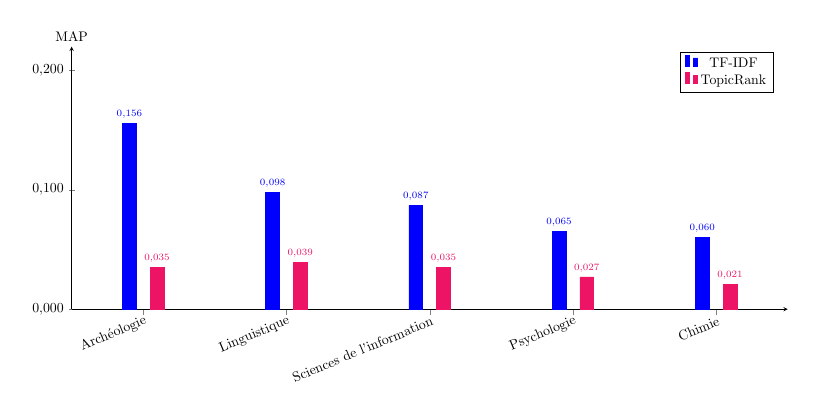
\begin{tikzpicture}[scale=.5]
            \pgfkeys{/pgf/number format/.cd, use comma, fixed, fixed zerofill, precision=3}
            \begin{axis}[axis lines=left,
                         symbolic x coords={Archéologie, Linguistique, Sciences de l'information, Psychologie, Chimie},
                         xtick=data,
                         enlarge x limits=0.125,
                         x=.3\linewidth,
                         xticklabel style={anchor=east, xshift=.5em, yshift=-.25em, rotate=22.5},
                         nodes near coords,
                         nodes near coords align={vertical},
                         every node near coord/.append style={font=\scriptsize},
                         ytick={0, 0.100, 0.200, 0.300, 0.400, 0.500},
                         y=2.5\linewidth,
                         ymin=0,
                         ymax=0.22,
                         ybar=10pt,
                         ylabel=MAP,
                         ylabel style={at={(ticklabel* cs:1)},
                                       anchor=south,
                                       rotate=270}]
              \addplot[Blue,
                       fill=Blue] coordinates{
                (Archéologie, 0.156)
                (Linguistique, 0.098)
                (Sciences de l'information, 0.087)
                (Psychologie, 0.065)
                (Chimie, 0.060)
              };
              \addplot[WildStrawberry,
                       fill=WildStrawberry] coordinates{
                (Archéologie, 0.035)
                (Linguistique, 0.039)
                (Sciences de l'information, 0.035)
                (Psychologie, 0.027)
                (Chimie, 0.021)
              };
              \legend{TF-IDF, TopicRank}
            \end{axis}
          \end{tikzpicture}
        }
      \end{figure}
    \end{minipage}\hfill
    \begin{minipage}{.45\linewidth}
      \begin{figure}
        \centering
        \subfigure[\texttt{(NOM | ADJ)+}]{
          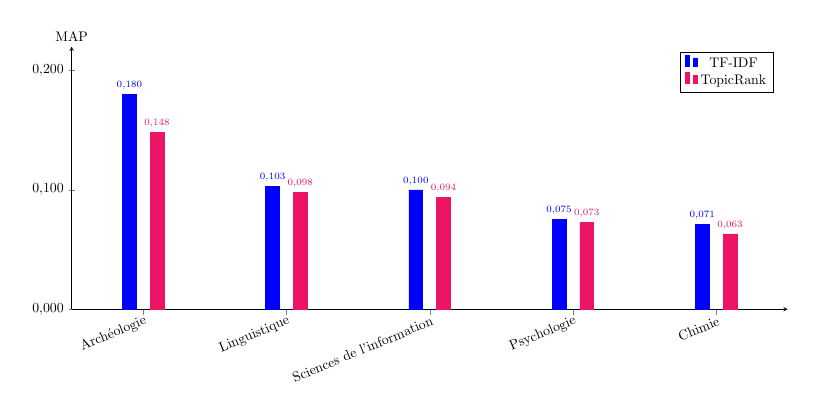
\begin{tikzpicture}[scale=.5]
            \pgfkeys{/pgf/number format/.cd, use comma, fixed, fixed zerofill, precision=3}
            \begin{axis}[axis lines=left,
                         symbolic x coords={Archéologie, Linguistique, Sciences de l'information, Psychologie, Chimie},
                         xtick=data,
                         enlarge x limits=0.125,
                         x=.3\linewidth,
                         xticklabel style={anchor=east, xshift=.5em, yshift=-.25em, rotate=22.5},
                         nodes near coords,
                         nodes near coords align={vertical},
                         every node near coord/.append style={font=\scriptsize},
                         ytick={0, 0.100, 0.200, 0.300, 0.400, 0.500},
                         y=2.5\linewidth,
                         ymin=0,
                         ymax=0.22,
                         ybar=10pt,
                         ylabel=MAP,
                         ylabel style={at={(ticklabel* cs:1)},
                                       anchor=south,
                                       rotate=270}]
              \addplot[Blue,
                       fill=Blue] coordinates{
                (Archéologie, 0.180)
                (Linguistique, 0.103)
                (Sciences de l'information, 0.100)
                (Psychologie, 0.075)
                (Chimie, 0.071)
              };
              \addplot[WildStrawberry,
                       fill=WildStrawberry] coordinates{
                (Archéologie, 0.148)
                (Linguistique, 0.098)
                (Sciences de l'information, 0.094)
                (Psychologie, 0.073)
                (Chimie, 0.063)
              };
              \legend{TF-IDF, TopicRank}
            \end{axis}
          \end{tikzpicture}
        }
      \end{figure}
    \end{minipage}

    \begin{minipage}{.45\linewidth}
      \begin{figure}
        \centering
        \subfigure[Candidats termes]{
          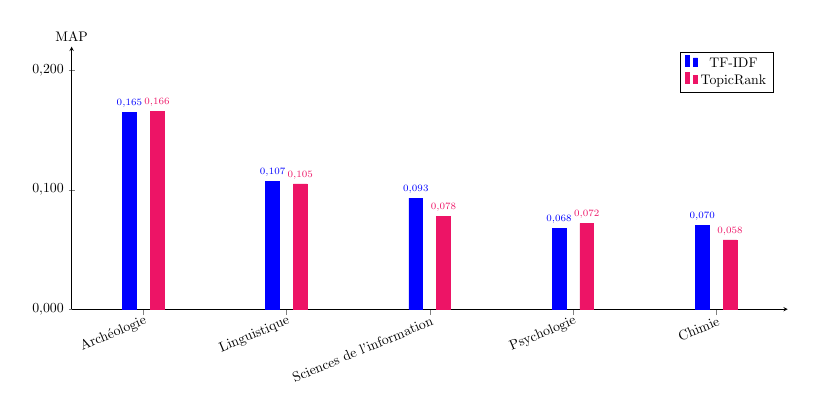
\begin{tikzpicture}[scale=.5]
            \pgfkeys{/pgf/number format/.cd, use comma, fixed, fixed zerofill, precision=3}
            \begin{axis}[axis lines=left,
                         symbolic x coords={Archéologie, Linguistique, Sciences de l'information, Psychologie, Chimie},
                         xtick=data,
                         enlarge x limits=0.125,
                         x=.3\linewidth,
                         xticklabel style={anchor=east, xshift=.5em, yshift=-.25em, rotate=22.5},
                         nodes near coords,
                         nodes near coords align={vertical},
                         every node near coord/.append style={font=\scriptsize},
                         ytick={0, 0.100, 0.200, 0.300, 0.400, 0.500},
                         y=2.5\linewidth,
                         ymin=0,
                         ymax=0.22,
                         ybar=10pt,
                         ylabel=MAP,
                         ylabel style={at={(ticklabel* cs:1)},
                                       anchor=south,
                                       rotate=270}]
              \addplot[Blue,
                       fill=Blue] coordinates{
                (Archéologie, 0.165)
                (Linguistique, 0.107)
                (Sciences de l'information, 0.093)
                (Psychologie, 0.068)
                (Chimie, 0.070)
              };
              \addplot[WildStrawberry,
                       fill=WildStrawberry] coordinates{
                (Archéologie, 0.166)
                (Linguistique, 0.105)
                (Sciences de l'information, 0.078)
                (Psychologie, 0.072)
                (Chimie, 0.058)
              };
              \legend{TF-IDF, TopicRank}
            \end{axis}
          \end{tikzpicture}
        }
      \end{figure}
    \end{minipage}\hfill
    \visible<2->{\cornersize{0.1}\Ovalbox{
      \begin{minipage}{.5\linewidth}
        \begin{itemize}
          \item<2->{Même échelle de difficulté pour TF-IDF et TopicRank}
          \item<3->{Meilleur stabilité du TF-IDF}
          \begin{itemize}
            \item[$\Rightarrow$]{Spécificité IDF}
          \end{itemize}
          \item<3->{TopicRank dépend de la qualité des candidats}
        \end{itemize}
      \end{minipage}
    }}
  \end{frame}

  \begin{frame}{Expérience}
    \framesubtitle{}

    \uncover<1,2,3,4,5>{Observations~:}
    \begin{enumerate}
      \item<2>{Même échelle de difficulté pour les deux méthodes}
      \item<3>{Meilleure stabilité du TF-IDF en fonction de la qualité des
            candidats}
      \begin{itemize}
        \item[$\Rightarrow$]{Les candidats retournés sont les candidats
                             spécifiques}
      \end{itemize}
      \item<4>{Plus les candidats sont de bonne qualité, plus TopicRank est
            compétitif avec TF-IDF}
    \end{enumerate}

    Conclusions~:
    \begin{enumerate}
      \item<2,6>{Il y a bien une influence de la discipline sur la difficulté de
            l'extraction de termes-clés}
      \item<3,6>{La présence ou non, dans les termes-clés, de mots à usage courant dans le language de la
            discipline est un facteur influent}
      \begin{itemize}
        \item[$\rightarrow$]{\textit{\og{}\underline{réaction}
                             sonochimique\fg{}, \og{}\underline{réaction}
                             électrochimique\fg{}, etc.}}
      \end{itemize}
      \item<4->{La cohésion au sein du texte est un facteur influent}
    \end{enumerate}

    \visible<5>{
      \begin{textblock*}{\textwidth}(0\textwidth, -0.907\textheight)
        \setbeamertemplate{blocks}[rounded][shadow=true]

        \begin{exampleblock}{\footnotesize Variabilité du Gravettien de Kostienki
                             (bassin moyen du Don) et des territoires
                             associés}\scriptsize
          \justifying{
            Dans la région de Kostienki-Borschevo, on observe l'expression, à ce
            jour, la plus orientale du modèle européen de l'évolution du
            Paléolithique supérieur. Elle est différente à la fois du modèle
            Sibérien et du modèle de l'Asie centrale. Comme ailleurs en Europe, le
            Gravettien apparaît à Kostienki vers 28 ka (Kostienki 8 /II/). Par la
            suite, entre 24-20 ka, les techno-complexes gravettiens sont
            représentés au moins par quatre faciès dont deux, ceux de Kostienki
            21/III/ et Kostienki 4 /II/, ressemblent au Gravettien occidental et
            deux autres, Kostienki-Avdeevo et Kostienki 11/II/, sont des faciès
            propres à l'Europe de l'Est, sans analogie à
            l'Ouest.\\\vspace{.5em}

            \underline{Descripteurs (termes-clés)~:} Europe, Kostienko,
            Borschevo, variation, typologie, industrie osseuse, industrie
            lithique, Europe centrale, Avdeevo, Paléolithique
            supérieur,
            Gravettien.\\\hfill\underline{\tiny\textit{Archéologie}}
          }
        \end{exampleblock}

        \vspace{.1em}

        \begin{exampleblock}{\footnotesize Etude d'un condensat acide
                             isocyanurique-urée-formaldéhyde}\scriptsize
          \justifying{
            La synthèse d'un condensat acide isocyanurique-urée-formaldéhyde
            utilisant la pyridine en tant que solvant a été effectuée par réaction
            sonochimique.\\\vspace{.5em}

            \underline{Descripteurs (termes-clés)~:} Réaction sonochimique,
            hétérocycle azote, cycle 6 chaînons,
            ether.\\\hfill\underline{\tiny\textit{Chimie}}
          }
        \end{exampleblock}
      \end{textblock*}
    }
  \end{frame}

